%%
%% This is file `mcmthesis-demo.tex',
%% generated with the docstrip utility.
%%
%% The original source files were:
%%
%% mcmthesis.dtx  (with options: `demo')
%%
%% -----------------------------------
%%
%% This is a generated file.
%%
%% Copyright (C)
%%       2010 -- 2015 by Zhaoli Wang
%%       2014 -- 2019 by Liam Huang
%%       2019 -- present by latexstudio.net
%%
%% This work may be distributed and/or modified under the
%% conditions of the LaTeX Project Public License, either version 1.3
%% of this license or (at your option) any later version.
%% The latest version of this license is in
%%   http://www.latex-project.org/lppl.txt
%% and version 1.3 or later is part of all distributions of LaTeX
%% version 2005/12/01 or later.
%%
%% This work has the LPPL maintenance status `maintained'.
%%
%% The Current Maintainer of this work is Liam Huang.
%%
%%
\documentclass{mcmthesis}
\mcmsetup{CTeX = false,    % 使用 CTeX 套装时,设置为 true
          tcn = \textcolor{black}{2409529}, problem = \textcolor{black}{E},
          sheet = true, titleinsheet = true, keywordsinsheet = true,
          titlepage = false, abstract = false}
        
\usepackage{newtxtext}     % \usepackage{palatino}
\usepackage[backend=bibtex]{biblatex}   % for RStudio Complie
\usepackage{tocloft}
\setlength{\cftbeforesecskip}{6pt}
\renewcommand{\contentsname}{\hspace*{\fill}\Large\bfseries Contents \hspace*{\fill}}
\usepackage{enumitem}

% Reduce spacing in itemize environment
\setlist[itemize]{itemsep=0pt, parsep=0pt}

\setlength{\parskip}{0.5em} % Adjust the 0.5em to the desired space
\setlist[enumerate]{itemsep=0pt}
\usepackage{subcaption}
\title{Navigating the Turbulent Waters}
% \author{\small \href{http://www.latexstudio.net/}
%   {\includegraphics[width=7cm]{mcmthesis-logo}}}
\date{\today}

\begin{document}

\begin{abstract}
    \paragraph{ }In response to the increasing frequency of global extreme weather events, property owners and insurers are confronting crises unprecedented in scale. This has prompted a fundamental reassessment and redevelopment of traditional risk assessment models and underwriting strategies, leading to our creation of three innovative models: PANDRA, the Real Estate Development Insurance Model, and E-SVM-HCP. Each model offers a detailed risk evaluation and decision-making framework.

    For Model 1, this \textbf{PANDRA} model decomposes into a demand model and a risk model, identifying six critical \textbf{fuzzy comprehensive evaluation} factors—such as the rate of natural disasters and urban density—and uses the \textbf{entropy weight method} to determine weight sets Through refinement of \textbf{membership functions} and \textbf{comprehensive evaluation models}, PANDRA yields the following needs assessment for Vermont: \textit{[Highly Needed: 0.022, Needed: 0.246, Optional: 0.533, Less Necessary: 0.281, Not Needed: 0.026]}.The \textbf{risk degree} for Vermont is represented by this matrix:\textit{[Very High Risk: 0.061, High Risk: 0.406, Moderate Risk: 0.370, Low Risk: 0.146, Very Low Risk: 0.017]}.The analysis assists insurance companies in making informed policy underwriting choices by evaluating these indices to balance demand and risk.

    For Model 2, the \textbf{Real Estate Development Insurance Model} employs \textbf{Analytic Hierarchy Process (AHP)} to systematically evaluate factors influencing real estate development within the insurance framework. Through a \textbf{calculated Consistency Ratio (CR)}, it offers nuanced insights into the suitability of real estate projects, with \textbf{grey forecasting} and \textbf{relational analysis to analyzing data correlation}, thereby forecasting development trajectories and assessing the interplay of different factors.

    For Model 3, \textbf{E-SVM-HCP}, equips community leaders with a \textbf{robust SVM-based tool} for historic preservation decisions. It evaluates cultural significance and potential economic benefits to prioritize preservation, optimizing \textbf{feature engineering} and \textbf{kernel functions} to address the unique challenges of cultural heritage decision-making, blending precision and reverence for history.

    Our integrative approach through PANDRA, the Real Estate Development Insurance Model, and E-SVM-HCP, provides a robust framework for risk assessment and cultural preservation. We've crafted a meticulous strategy involving \textbf{sensitivity analyses} to reinforce model resilience and policy dynamism. Our synthesized efforts culminate in a strategic plan communicated through a \textbf{community letter}, outlining a cost-effective and timeline-conscious approach to preserving culturally significant landmarks while embracing future development and maintaining community heritage. This multifaceted plan sets a precedent for future work that requires adaptability, proactive engagement, and a thorough understanding of the intricate balance between heritage conservation and modernization demands.
    
    \begin{keywords}
        Climate Change, Property Insurance, Analytic Hierarchy Process, Grey Forecasting, E-SVM-HCP
    \end{keywords}

\end{abstract}

\maketitle

%% Generate the Table of Contents, if it's needed.
% \renewcommand{\contentsname}{\centering Contents}
\tableofcontents        % 若不想要目录, 注释掉该句
\thispagestyle{empty}

\newpage

\section{Introduction}

\subsection{Problem Background}

Climate change is not a specter on the horizon but a storm we are living through. The property insurance sector, long predicated on stability and predictability, now grapples with the capricious nature of a warming planet. As extreme weather events become more frequent and severe, insurers and property owners alike face a dual crisis: soaring premiums and a burgeoning insurance protection gap that threatens to leave vast swathes of our cultural and economic heritage uninsured and unprotected. This complex landscape requires a radical rethinking of traditional risk assessment models and underwriting strategies, as well as a proactive approach to the preservation of properties that embody significant cultural, historical, and economic value.

Scholars such as Williamson and Hudson (2021) have highlighted the increasing volatility in insurance claim patterns related to climate-induced disasters, emphasizing the need for a paradigm shift in risk modeling and financial planning within the industry \cite{1}. Furthermore, the work of Fisher and Kumar (2022) has brought attention to the growing insurance protection gap, particularly in regions highly susceptible to climate change, underscoring the urgency of developing more inclusive and resilient insurance frameworks \cite{2}.


\begin{figure}[h] 
    \centering
    \includegraphics[width=12cm]{fig_int.jpg}
    \caption{Extreme Weather} \label{fig_int}
\end{figure}

\subsection{Restatement of the Problem}

Given the increasing severity of extreme weather events and their consequential impact on the property insurance sector, our team is dedicated to addressing this multifaceted challenge by:

\begin{enumerate}
    \item \textbf{Modeling for Insurance Decision-Making:} Developing a robust model to guide insurance companies in making informed decisions about underwriting policies in areas prone to extreme weather. The model aims to define the conditions under which companies should underwrite policies, identify the appropriate times to accept risks, and explore ways property owners can influence these decisions.
    
    \item \textbf{Adapting the Insurance Model for Real Estate Decisions:} Tailoring the insurance model to assess key considerations in real estate development, such as determining suitable locations, construction methodologies, and the feasibility of building projects in the context of changing insurance landscapes.
    
    \item \textbf{Creating a Preservation Model for Community Leaders:} Developing a comprehensive preservation model that aids community leaders in recognizing and safeguarding structures of cultural, historical, economic, or community importance. This model will serve as a tool for determining the necessary measures to protect and preserve the integral buildings within their communities.
    
    \item \textbf{Communicating with the Community:} Crafting a detailed one-page letter to the community, outlining a strategic plan, timeline, and financial proposal for the future preservation of treasured landmarks. This communication will reflect the insights garnered from the insurance and preservation models, ensuring a well-informed and community-centered approach.
\end{enumerate}

\subsection{Our Work: Analyzing Risk and Informing Decision-Making}
This paper introduces a tripartite model framework that is engineered to redefine the paradigm of property insurance underwriting and cultural heritage preservation amidst the evolving challenges posed by climate change. Our approach systematically amalgamates advanced statistical techniques with forward-looking climate projection data, thereby transcending traditional actuarial methodologies to furnish a granular risk assessment.

\begin{figure}[h]
    \centering
    \includegraphics[width=12cm]{Design.png}
    \caption{Flowchart of our study}
    \label{fig:SystemDesign}
\end{figure}

\subsection{Assumptions and Justifications}

Considering the complex nature of modeling insurance needs in the face of climate change, we present our assumptions followed by their justifications to bolster the model's validity:

\begin{itemize}
    \item[$\blacktriangleright$] \textbf{Assumption 1: Uniformity in Catastrophe Definition.} 
        \begin{itemize}
            \item[$\vartriangleright$] \textit{Justification:} Standardizing the definition of extreme-weather events ensures data comparability and model coherence, providing a consistent framework for analysis.
        \end{itemize}
    
    \item[$\blacktriangleright$] \textbf{Assumption 2: Stability of Economic Parameters.}
        \begin{itemize}
            \item[$\vartriangleright$] \textit{Justification:} Economic factors such as inflation rates and property values are considered stable in the short term, sharpening the model's focus on weather-related variables.
        \end{itemize}
    
    \item[$\blacktriangleright$] \textbf{Assumption 3: Homogeneity in Risk Perception.}
        \begin{itemize}
            \item[$\vartriangleright$] \textit{Justification:} Assuming a uniform risk perception among stakeholders allows the model to provide universally applicable guidelines, free from individual biases.
        \end{itemize}
    
    \item[$\blacktriangleright$] \textbf{Assumption 4: Consistency in Policy Application.}
        \begin{itemize}
            \item[$\vartriangleright$] \textit{Justification:} This assumption is crucial for deriving actionable insights across regions, facilitating insurance companies to implement uniform underwriting policies.
        \end{itemize}
\end{itemize}

\section{Notations}
\begin{table}[h]
    \centering
    \caption{List of Notations}
    \begin{tabular}{|c|c|}
    \hline
    \textbf{Notation} & \textbf{Description} \\
    \hline
    $U$ & Determinant Ensemble \\
    $V$ & Appraisal Lexicon \\
    $A$ & Significance Aggregator \\
    $X_{ij}$ & Original value of the $j$-th indicator for the $i$-th object \\
    $X'_{ij}$ & Normalized value of the $j$-th indicator for the $i$-th object \\
    $Z_{ij}$ & Standardized value of the $j$-th indicator for the $i$-th object \\
    $P_{ij}$ & Probability of the $j$-th indicator for the $i$-th object \\
    $E_j$ & Entropy of the $j$-th indicator \\
    $W_j$ & Entropic weight of the $j$-th indicator \\
    $V_{\text{maximal}}$ & Transformed maximal-type value \\
    $V_{\text{minimal}}$ & Original minimal-type value \\
    $\Phi(z)$ & Cumulative distribution function for a normal distribution \\
    $f(x; \mu, \sigma)$ & Probability density function of the normal distribution \\
    \hline
    \end{tabular}
    \label{table:notations}
    \end{table}
    
\noindent where we define the main parameters while specific value of those parameters will be given later.

\section{Model Overview}

\subsection{Panoramic Insurance Needs and Risk Assessment Model (PANDRA)}
The PANDRA model is designed to address the insurance industry's challenges in underwriting policies in areas prone to extreme weather events. As climate change escalates the severity and frequency of such events, PANDRA aims to provide a robust framework to assess the risks and potential claims costs in different geographic regions. The model integrates risk assessment, sustainability considerations, and the influence of property owners into a holistic view, ensuring long-term viability for insurance companies while serving the needs of property owners. By incorporating ample factorsmics, PANDRA offers a comprehensive tool for insurers to balance risk, profitability, and sustainability in their policy underwriting decisions.

\subsection{Analytic Hierarchy Process for Real Estate Development Insurance Model}
As the insurance landscape evolves, real estate decisions must be made with deliberation, ensuring properties are resilient and strategically placed. This model employs the Analytic Hierarchy Process (AHP) to guide developers in identifying optimal sites for construction, taking into account the changing dynamics of property insurance. The model evaluates factors such as climate resilience, risk mitigation strategies, community involvement, and sustainable development practices. By providing a structured decision-making framework, the model aids developers and community leaders in making informed choices about where, how, and whether to build, ensuring future properties are aligned with the principles of resilience and sustainability in the face of extreme weather events.

\subsection{Historical Cultural Preservation Model using Enhanced SVM (E-SVM-HCP)}
In regions where extreme weather events are prevalent, community leaders face the challenge of preserving buildings with cultural, historical, economic, or community significance. The E-SVM-HCP model is an optimized SVM framework tailored for this purpose. It classifies significant buildings for preservation based on a multifaceted evaluation of factors like historical value, cultural significance, economic impact, and legal protection. The model's customized kernel function and non-linear penalty for classification errors ensure sensitivity to the unique aspects of cultural preservation. E-SVM-HCP provides community leaders with a data-driven tool to make decisions on preserving their cultural heritage, considering the intricate interplay between preservation value and the threats posed by extreme weather conditions.

\section{Model Application Sites Analysis}
\textbf{Rationale for Location Selection:} Our models are applied to regions distinctly impacted by climate phenomena, as depicted in the provided climatic map Figure\ref{fig:climatic_zones}. These areas are prone to extreme weather events, influencing our decision to assess the viability of insurance underwriting and the necessity for preservation efforts.

\textbf{Analysis of Climatic Zones:}
\begin{itemize}
    \item \textbf{Inter-tropical Convergence Zone (ITCZ):} Characterized by heavy precipitation, the ITCZ's dynamic weather patterns necessitate an adaptable insurance framework to manage the heightened risk of flooding.
    \item \textbf{Subtropical and Extratropical Storms:} These regions experience a high frequency of cyclonic activity, underscoring the importance of robust insurance models to mitigate the financial impact on property and heritage sites.
\end{itemize}

\textbf{Justification for Model Deployment:}
\begin{enumerate}
    \item In the \textit{Subtropics}, our models capitalize on the patterns of subtropical storms to predict potential damages, aiding insurers in calculating premiums accurately.
    \item \textit{Mid-latitude Westerlies} region's exposure to extratropical storms informs our preservation model, emphasizing structural resilience in historic landmarks.
\end{enumerate}

\textbf{Incorporating Geographic Specificity:}
The models' parameters are fine-tuned to reflect the unique climatic conditions of each zone, ensuring precise assessments tailored to the local meteorological realities.

Based on the above analysis, we selected Auckland, New Zealand, and Vermont, USA. Our selection of these two sites, as model application sites is underpinned by a robust rationale driven by their distinct vulnerability to extreme weather events in different climatic zones. Auckland, representing the Inter-tropical Convergence Zone (ITCZ) with its heavy precipitation and dynamic weather patterns, highlights the critical need for adaptable insurance frameworks to manage heightened flood risks effectively. Conversely, Vermont's exposure to subtropical and extratropical storms underscores the importance of deploying robust insurance models and promoting structural resilience in historic landmarks within the Mid-latitude Westerlies region.

\textbf{Figure Reference:}
\begin{figure}[h]
    \centering
    \includegraphics[width=8cm]{NewZealand.png}
    \caption{Climatic zones and storm paths influencing model application sites.}
    \label{fig:climatic_zones}
\end{figure}

\section{Panoramic Insurance Needs and Risk Assessment Model (PANDRA)}

This section introduces the Panoramic Insurance Needs and Risk Assessment Model (PANDRA), a comprehensive framework developed to assist insurance companies in navigating the complexities of underwriting policies in regions prone to extreme weather events. PANDRA synergistically integrates two distinct but interconnected components: the Panoramic Insurance Needs (PAN) model and the Disaster Risk Assessment (DRA) model. This integration facilitates a holistic approach to insurance needs and risk assessment, taking into account a wide spectrum of factors from natural disaster frequency and severity to socioeconomic dynamics, geographic characteristics, and the influence of property owners' actions.

\begin{figure}[h]
    \centering
    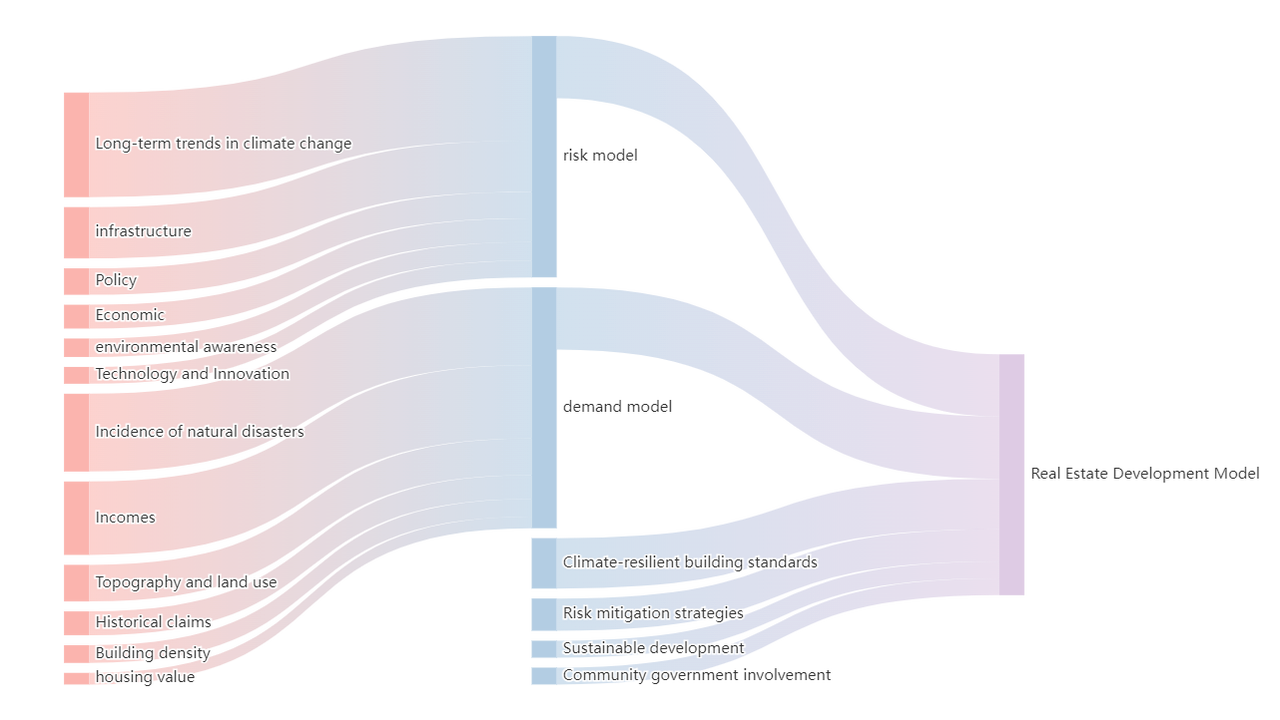
\includegraphics[width=12cm]{PANDRA.png}
    \caption{PANDRA Model} \label{PANDRA}
\end{figure}

\subsection{Panoramic Insurance Needs (PAN)}
\subsubsection{Constituent Elements Articulation}
The formulation of the Panoramic Insurance Needs (PAN) model revolves around a meticulously engineered framework, encompassing a spectrum of determinants conceptualized to delineate the multifaceted nature of insurance necessities and associated risks.

\textbf{1. Determinant Ensemble (U)}
The Determinant Ensemble, representing a curated compendium of influential factors, is the linchpin of the PAN model. It encapsulates:
\begin{enumerate}
    \item The \textbf{Natural Disaster Incidence Rate (U1)}, serving as a barometer for gauging the vulnerability of regions to catastrophic events.
    \item The \textbf{Urban Density Index (U2)}, which mirrors the potential compound risk in densely populated areas.
    \item The \textbf{Economic Vitality Indicator (U3)}, reflecting the financial robustness and insurance-affordability of demographics.
    \item The \textbf{Asset Valuation Parameter (U4)}, indicative of the monetary stakes involved and the consequent insurance stakes.
    \item The \textbf{Historical Claims Chronicle (U5)}, offering empirical insights into the claim patterns and risk proneness of sectors.
    \item The \textbf{Topographic and Land Utilization Synopsis (U6)}, painting a vivid picture of how geographical contours and anthropogenic land use sculpt the insurance landscape.
\end{enumerate}

\textbf{2. Appraisal Lexicon (V)}
The Appraisal Lexicon constitutes a graded spectrum of evaluative terms, stratifying the insurance necessity from 'Highly Needed' to 'Not Needed', thereby instilling a nuanced granularity into the assessment, as demonstrated in Figure~\ref{fig::Appraisal-Level}.

\begin{figure}[h]
    \centering
    \includegraphics[width=12cm]{Needed.png}
    \caption{Appraisal Level} \label{fig::Appraisal-Level}
\end{figure}

\textbf{3. Significance Aggregator (A)}
The Significance Aggregator is emblematic of the relative prominence of each determinant within the ensemble. Rooted in the entropy-weighting method, it is a testament to an empirical approach to ascertaining the weighted significance, ensuring an unbiased and data-driven synthesis of determinants.

\subsubsection{Entropic Weight Ascertainment for Significance Aggregator (A)}
The construction of the Significance Aggregator (A) within the PAN framework incorporates an advanced entropic weighting methodology, designed to objectively quantify the influence of each determinant. This rigorous approach ensures that the composite assessment reflects the inherent importance of each constituent factor, thereby enhancing the precision of the model. The procedure unfolds through several systematic phases:

1. Normalization of the Primitive Matrix

Our original matrix consists of Determinant Ensemble(U) from U1 to U6.To harmonize the diverse nature of the indicators and convert them into a unified format conducive for further analysis, the primitive matrix is normalized, ensuring that each indicator is transformed into a \textit{maximal-type} indicator, representing a paradigm where higher values connote more favorable outcomes.
\begin{equation}
X'_{ij} = \frac{X_{ij} - \min(X_j)}{\max(X_j) - \min(X_j)}
\end{equation}
where $X_{ij}$ denotes the original value of the $j$-th indicator for the $i$-th object, and $X'_{ij}$ represents the normalized value.

2. Standardization of the Normalized Matrix

The normalized matrix undergoes a standardization process, ensuring comparability across different indicators and establishing a groundwork for subsequent probabilistic assessments.
\begin{equation}
Z_{ij} = \frac{X'_{ij}}{\sum_{i=1}^n X'_{ij}}
\end{equation}
where $Z_{ij}$ signifies the standardized value.

3. Probability Matrix Computation (P)

The standardized matrix is then utilized to construct a probability matrix (P), offering a refined structure for encapsulating the distribution characteristics of each indicator.
\begin{equation}
P_{ij} = \frac{Z_{ij}}{\sum_{j=1}^m Z_{ij}}
\end{equation}
where $P_{ij}$ symbolizes the probability of the $j$-th indicator for the $i$-th object.

4. Entropic Weight Calculation

The entropic weight for each indicator is calculated to quantitatively express its informational entropy, which intrinsically reflects the degree of disorder or randomness associated with the indicator's distribution. The entropic weight is a testament to the significance of each indicator within the overall assessment framework.
\begin{align}
E_j &= -k \sum_{i=1}^n P_{ij} \ln(P_{ij}) \\
W_j &= \frac{1 - E_j}{m - \sum_{j=1}^m E_j}
\end{align}
where $E_j$ is the entropy of the $j$-th indicator, $k = \frac{1}{\ln(n)}$ is a constant, and $W_j$ is the entropic weight of the $j$-th indicator.

\subsection{Enhanced Probabilistic Calibration of Membership Functions}
Our model adopts a sophisticated probabilistic approach to calibrate membership functions that categorize risk levels and insurance necessity. This calibration is particularly critical in the context of extreme weather events and their impact on property insurance.

\textbf{Empirical Data Analysis}
We initiate the process by calculating the mean, $\mu$, and standard deviation, $\sigma$, for each risk determinant such as the rate of occurrence of natural disasters. These statistics are essential for constructing the membership functions based on the cumulative distribution function (CDF) of the normal distribution:

\begin{equation}
\Phi(z) = \frac{1}{2}\left[1 + \text{erf}\left(\frac{z - \mu}{\sigma\sqrt{2}}\right)\right],
\end{equation}
where $\Phi(z)$ represents the CDF for a value $z$ in the normal distribution, and $\text{erf}$ is the error function which integrates Gaussian distributions.

\textbf{Normal Distribution and Membership Functions}
To derive the membership values, we consider the normal distribution probability density function (PDF):

\begin{equation}
    f(x; \mu^\prime, \sigma^\prime) = \frac{1}{\sigma^\prime\sqrt{2\pi}}e^{(-\frac{(x - \mu^\prime)^2}{2\sigma^\prime2})}, \mu' = \Phi(z),
\end{equation}
and integrate this function over the intervals corresponding to the fuzzy sets of insurance necessity, from 'Highly Needed' to 'Not Needed'. This integration is visualized in Figure \ref{fig:math_rel}, where the area under the curve represents the probability associated with each category of necessity.

\textbf{Rationale Behind $\sigma^\prime$ Selection:}
The selection of $\sigma^\prime = 0.1$ is informed by the empirical rule which indicates that, for a normal distribution, approximately 95.45\% of the data falls within two standard deviations ($2\sigma^\prime$) from the mean ($\mu^\prime$). This statistical insight is applied to ensure that the 'optional' insurance necessity range, defined from 0.4 to 0.6, corresponds to the central portion of the distribution where most data points are concentrated.


\textbf{Derivation of Membership Values}
Integrating the PDF over the necessary intervals, we obtain the membership values for each category:

\begin{equation}
\int_{a}^{b} f(x; \mu, \sigma) dx,
\end{equation}
where $[a, b]$ defines the interval for each category ([0, 0.2], [0.2, 0.4], [0.4, 0.6], [0.6, 0.8], [0.8, 1]) correspond to categories that seem to represent different levels of necessity for insurance, ranging from "Not Needed" to "Highly Needed.". These values are then normalized to sum up to unity across all categories.

\begin{figure}[h]
\centering
\includegraphics[width=0.75\textwidth]{F_Model1.png}
\caption{Mathematical relationship between input values and insurance needs.}
\label{fig:math_rel}
\end{figure}

\subsubsection{Establishment of the Fuzzy Comprehensive Evaluation Matrix (R)}
In the Synoptic Appraisal of Insurance Imperatives and Risk Stratification (PAN) model, the establishment of the Fuzzy Comprehensive Evaluation Matrix (R) is pivotal for elucidating the intricate interdependencies among the determinant factors and the graded insurance necessity spectrum. The construction of this matrix involves the transformation of raw values into a maximal-type configuration to resonate with the model's assessment philosophy where higher values signify augmented necessity or risk.

The synthesis of this matrix with the probabilistic calibration of membership functions ensures a robust, data-driven approach to insurance risk assessment within diverse climatic contexts. To construct the matrix \( R \), values are determined based on a combination of empirical data retrieval and expert assessment. The matrix reflects the influence and interplay of various factors, quantified as follows:

\begin{itemize}
    \item \textbf{Natural Disaster Frequency}: Represented by the number of meteorological disasters occurring per month.
    \item \textbf{Building Density}: Defined as the ratio of the urban population to the urban area, reflecting the concentration of buildings in a given area.
    \item \textbf{Economic Development Indicators}: Comprised of per capita national income, median family income, and the unemployment rate among residents.
    \item \textbf{Value of Housing}: Indicated by the average local house price, offering a measure of the financial stakes involved.
    \item \textbf{Historical Claim Data}: Derived from data provided by the New Zealand Insurance Commission, reflecting past claim patterns and frequencies.
    \item \textbf{Terrain and Land Use}: Factors such as the length of rivers multiplied by the area of both banks to represent flood plains, coastline length, tidal flat area, and low-lying areas prone to flooding are considered to assess the risk associated with topography and land use.
\end{itemize}

Each factor is assigned a value based on the aforementioned criteria, and these values are then populated into the matrix \( R \). The unit of measurement for each factor is tailored to its nature and the most common metrics used in its assessment, ensuring that the matrix offers a nuanced and comprehensive view of the risk landscape.

\textbf{Transformation into Maximal-Type Values}
Special attention is paid to ensure that all values are represented in a maximal-type format. For determinants where lower values traditionally represent a more favorable scenario (minimal-type) after normalization, a transformation is employed to invert the scale, thus aligning with the maximal-type paradigm. This is achieved through the equation:
\begin{equation}
V_{maximal} = 1 - V_{minimal}
\end{equation}
where $V_{maximal}$ represents the transformed maximal-type value, and $V_{minimal}$ is the original minimal-type value.

\subsubsection{Synthesis of the Comprehensive Evaluation Model}
The synthesis of the Comprehensive Evaluation Model within PANDRA (Panoramic Insurance Needs and Risk Assessment Model) is executed via an advanced fuzzy synthetic evaluation method. This technique employs the fusion of a fuzzy relation matrix \( R \) and a weight vector \( A \), materializing into a fuzzy result vector \( B \), which encapsulates the graded necessity of insurance across various predefined categories. 

Executing this synthesis necessitates a meticulous matrix operation, symbolized by \( \circ \), which is defined as:
\begin{equation}
B = A \circ R = \left( \max_{i} \min(a_{i}, r_{ij}) \right)_{j=1}^{m}
\end{equation}
Here, \( A = (a_1, a_2, \ldots, a_n) \) is the weight vector representing the importance of each criterion, and \( R \) is the fuzzy relation matrix composed of membership grades assigned to each criterion across different insurance necessity levels. The vector \( B \) is thus a composite fuzzy assessment, reflecting the confluence of each determinant's weighted influence.

The mathematical operation \( \max_{i} \min(a_{i}, r_{ij}) \) underpins the decision-making rule within PANDRA, selecting the maximal element from the minimal pairs formed by the corresponding weights and relation grades. This max-min operator is a hallmark of fuzzy logic, offering a means to accommodate the inherent imprecision within the decision-making context.

The resultant vector \( B \), with components \( b_j \), signifies the aggregate degree to which the ensemble of determinants correlates with each evaluative term within the insurance necessity lexicon. The highest value within \( B \) dictates the ultimate appraisal, denoting the most fitting category of insurance necessity given the prevailing conditions.

\subsection{DRA Module: Disaster Risk Assessment}
The DRA (Disaster Risk Assessment) module, following the structured approach of the PAN model in PANDRA, focuses on analyzing and quantifying the multifaceted dimensions of disaster-related risks impacting insurance. This module integrates the assessment of policy and response capacity, financial markets and investment returns, infrastructure robustness, environmental consciousness, technological and innovation indices, as well as the implications of climate change and long-term trends.

  \begin{figure}[h]
    \centering
    \begin{minipage}{.5\textwidth}
        \centering
        \includegraphics[width=.9\linewidth]{US1.png} % Example image
        \label{fig:vermont}
    \end{minipage}%
    \begin{minipage}{.5\textwidth}
        \centering
        \includegraphics[width=.9\linewidth]{US2.png} % Example image
        \label{fig:texas}
    \end{minipage}
    \label{fig::USA-storm}
    \caption{USA Storm Events}
\end{figure}

%   The DRA module's implementation within the PANDRA framework incorporates data analysis of storm events in the United States, as represented in Figure above. These visualizations underscore the disparate impact of storm events across different states, which is a crucial factor in risk assessment for insurance underwriting.
  
\subsubsection{Modification and Integration of Determinants in DRA}
DRA modifies and integrates the determinant ensemble to encompass the specificities of disaster risk in the context of insurance:
\begin{enumerate}
    \item \textbf{Policy and Response Capacity (D1)}: Quantifies the effectiveness of local policies and disaster response strategies.
    \item \textbf{Financial Market Stability and Investment Returns (D2)}: Assesses the stability of local financial markets and potential impacts on insurance.
    \item \textbf{Infrastructure Robustness (D3)}: Evaluates the resilience of physical infrastructure against disasters.
    \item \textbf{Environmental Consciousness (D4)}: Measures the level of environmental awareness and its impact on disaster risk mitigation.
    \item \textbf{Technological and Innovation Index (D5)}: Gauges the contribution of technology and innovation to disaster risk reduction.
    \item \textbf{Climate Change and Long-term Trends (D6)}: Analyzes the effects of climate change and long-term environmental trends on disaster risks, incorporating a climate classification matrix.
\end{enumerate}

\subsubsection{Climate Classification Matrix in DRA}
The Climate Classification Matrix is crucial in DRA for reflecting the variability and complexity of climate impact on disaster risks, The following table shows the structure of our Climate Classification Matrix based on the PAN model:
% Table for Climate Classification Matrix
\begin{table}[h]
\centering
\caption{Climate Classification Matrix and Corresponding Membership Values}
\begin{tabular}{|c|c|}
\hline
\textbf{Climate Type} & \textbf{Membership Matrix} \\
\hline
Tropical Rainforest Climate & [0.7, 0.2, 0.1, 0, 0] \\
\hline
Temperate Oceanic Climate & [0.1, 0.1, 0.5, 0.2, 0.1] \\
\hline
Tropical Savanna Climate & [0.2, 0.4, 0.35, 0.05, 0] \\
\hline
Temperate Continental Climate & [0.2, 0.25, 0.5, 0.05, 0] \\
\hline
Tropical Desert Climate & [0.5, 0.3, 0.2, 0, 0] \\
\hline
Temperate Monsoon Climate & [0.3, 0.25, 0.25, 0.15, 0.05] \\
\hline
Tropical Monsoon Climate & [0.6, 0.3, 0.1, 0, 0] \\
\hline
Subarctic Coniferous Forest Climate & [0.4, 0.15, 0.25, 0.15, 0.05] \\
\hline
Mediterranean Climate & [0.1, 0.1, 0.4, 0.3, 0.1] \\
\hline
Polar Climate & [0.8, 0.2, 0, 0, 0] \\
\hline
Subtropical Monsoon and Humid Climate & [0.4, 0.2, 0.25, 0.1, 0.05] \\
\hline
Highland Climate & [0.5, 0.3, 0.2, 0, 0] \\
\hline
\end{tabular}
\label{table:ClimateClassificationMatrix}

\end{table}

\subsection{Application of the PANDRA Model}
The PANDRA model's application to Vermont and Auckland, New Zealand, leads to the following insights regarding insurance needs and underwriting risks.

\textbf{Vermont:} The insurance necessity in Vermont is categorized as 'optional', and the underwriting risk is identified as higher. The entropy method calculated the following weights for the determinants: [0.3231, 0.0794, 0.3549, 0.0986, 0.1010, 0.1519].

\textbf{Auckland, New Zealand:} In contrast, Auckland exhibits a clear need for insurance with a similar risk profile in underwriting. The same weights were calculated, suggesting that the determinants are consistent across the two regions.

Here are the Fuzzy Comprehensive Evaluation Matrices (R) for Vermont and Auckland:

% Table for Vermont


\begin{table}[h]
    \centering
    \caption{Fuzzy Comprehensive Evaluation Matrix (R) for Vermont}
    \resizebox{\linewidth}{!}{  
        \begin{tabular}{|l|c|c|c|c|c|}
            \hline
            \textbf{Determinants} & \textbf{Highly Needed} & \textbf{Needed} & \textbf{Optional} & \textbf{Less Needed} & \textbf{Not Needed} \\
            \hline
            Natural Disaster Incidence & 0.0015 & 0.1626 & 0.6826 & 0.1521 & 0 \\
            Urban Density & 0 & 0.0924 & 0.5849 & 0.2133 & 0.1094 \\
            Economic Development & 0 & 0.0098 & 0.3592 & 0.5832 & 0.0478 \\
            Property Valuation & 0.1583 & 0.6836 & 0.1567 & 0.0013 & 0 \\
            Historical Claims Data & 0.0069 & 0.3154 & 0.6157 & 0.0617 & 0.0002 \\
            Topography and Land Use & 0.0369 & 0.5473 & 0.4024 & 0.0135 & 0 \\
            \hline
        \end{tabular}
    } 
    \end{table}    

% Table for Auckland, New Zealand
\begin{table}[h]
\centering
\caption{Fuzzy Comprehensive Evaluation Matrix (R) for Auckland, New Zealand}
\resizebox{\linewidth}{!}{  
\begin{tabular}{|l|c|c|c|c|c|}
\hline
\textbf{Determinants} & \textbf{Highly Needed} & \textbf{Needed} & \textbf{Optional} & \textbf{Less Needed} & \textbf{Not Needed} \\
\hline
Natural Disaster Incidence & 0.0169 & 0.4349 & 0.5181 & 0.0301 & 0 \\
Urban Density & 0.1246 & 0.6779 & 0.1953 & 0.0022 & 0 \\
Economic Development & 0.0715 & 0.6329 & 0.2900 & 0.0056 & 0 \\
Property Valuation & 0.1065 & 0.6690 & 0.2217 & 0.0029 & 0 \\
Historical Claims Data & 0.0002 & 0.0647 & 0.6213 & 0.3073 & 0.0065 \\
Topography and Land Use & 0.2004 & 0.6776 & 0.1213 & 0.0008 & 0 \\
\hline
\end{tabular}
}
\end{table}

\begin{table}[h]
    \centering
    \caption{Necessity of Insurance}
    \begin{tabular}{@{}lccccc@{}}
    \toprule
                  & Highly Needed & Needed & Optiona & Less Needed & Not Needed \\ \midrule
    Vermont & 0.02239504 & 0.24574387 & 0.53323008 & 0.28146774 & 0.02609081 \\
    Auckland & 0.08169084 & 0.5943832 & 0.38886232 & 0.04333219 & 0.00068881 \\ \bottomrule
    \end{tabular}
    \end{table}
    
    \begin{table}[h]
    \centering
    \caption{Risk Levels}
    \begin{tabular}{@{}lccccc@{}}
    \toprule
                  & Highly Risk & Higher Risk & Medium Risk & Lower Risk & Very Low Risk\\ \midrule
    Vermont & 0.06056319 & 0.4058455 & 0.36969653 & 0.14644262 & 0.01744466 \\
    Auckland & 0.26430453 & 0.26804606 & 0.25264984 & 0.20930209 & 0.06555666 \\ \bottomrule
    \end{tabular}
    \end{table}

The final result drawn from these matrices indicates that while Vermont's insurance necessity is optional, Auckland requires insurance. Both regions show a considerable underwriting risk, but not at a level that would discourage insurers from offering coverage.

\subsection{Strategic Implications for Property Owners}

Given the PANDRA model's findings, property owners in regions like Vermont and Auckland are confronted with the strategic imperative to influence the underwriting decisions of insurance companies. The model's insights into the nuanced interplay of risk factors provide a roadmap for property owners to take proactive measures that could sway insurance companies to offer favorable policy terms.

\textbf{Mitigation Efforts to Influence Underwriting}
Property owners can undertake various mitigation strategies to reduce the perceived risk and therefore encourage insurance companies to underwrite policies. These strategies include:

\begin{itemize}
    \item \textbf{Infrastructure Upgrades:} Enhancing the resilience of property structures against extreme weather events, such as improving drainage systems to prevent flood damage or reinforcing structures to withstand high winds.
    \item \textbf{Adoption of Smart Technologies:} Implementing smart home technologies that can detect and prevent potential damages early, such as water sensors for leak detection and automated shut-off systems.
    \item \textbf{Community-Level Initiatives:} Participating in community-wide disaster preparedness programs and advocating for public infrastructure that mitigates the impact of natural disasters.
    \item \textbf{Environmental Stewardship:} Engaging in environmental conservation efforts that help mitigate climate change and thus reduce the frequency and severity of extreme weather events.
\end{itemize}

\textbf{Economic Incentives and Negotiation}
Economic incentives can be a potent tool for property owners to negotiate better insurance terms:

\begin{itemize}
    \item \textbf{Premium Discounts:} Seeking premium discounts for properties that have implemented recognized risk mitigation measures.
    \item \textbf{Policy Customization:} Working with insurers to customize policies that reflect the unique risk profile of the property, possibly resulting in lower premiums.
\end{itemize}


% \textbf{Model Application to Policy Determination}
% Applying the PANDRA model to the context of Vermont and Auckland, it becomes evident that insurance companies should underwrite policies under conditions where the risk is manageable and mitigated by proactive actions taken by property owners. The decision to take the risk hinges on a comprehensive analysis provided by models that consider the multifaceted nature of climate change and its impact on property insurance. The PANDRA model is instrumental in providing such analysis and helping insurers make informed decisions on policy underwriting.

% Table for PANDRA Model Application Conclusions
% \begin{table}[h]
% \centering
% \caption{PANDRA Model Application Conclusions}
% \begin{tabular}{lcc}
% \toprule
% \textbf{Location} & \textbf{Insurance Need} & \textbf{Underwriting Risk} \\
% \midrule
% Vermont & Optional & Higher \\
% Auckland, New Zealand & Needed & Higher \\
% \bottomrule
% \end{tabular}
% \end{table}


\section{Analytic Hierarchy Process for Real Estate Development Insurance Model}


    In the landscape of modern real estate development, accurately assessing risk and forecasting developmental trajectories is paramount. Our model harnesses the Analytic Hierarchy Process (AHP) and Grey Systems Theory to dissect and prioritize the insurance risk factors. AHP meticulously structures multifaceted criteria into a judgment matrix, facilitating a consistent evaluation of risk components as depicted in Figure \ref{fig:ahp_flow}. Grey Forecasting and Relational Analysis further our model's prowess by capturing the subtleties within incomplete data, enabling robust predictions in uncertain environments. These methods, synergistically applied, empower stakeholders to navigate the real estate sector's volatility effectively, with a particular emphasis on climate resilience and sustainable development.
    
    \begin{figure}[h]
    \centering
    \includegraphics[width=0.8\linewidth]{Model2.png}
    \caption{Analytic Hierarchy Process integrated with Grey System components.}
    \label{fig:ahp_flow}
    \end{figure}

\subsection{Judgment Matrix Construction and Consistency Evaluation}
The Analytic Hierarchy Process (AHP) is utilized to systematically analyze and prioritize the multifaceted criteria influencing real estate development decisions in the context of insurance risk management. These methodologies, when cohesively integrated, equip stakeholders to adeptly manage the complexities of the real estate sector. They particularly enhance decision-making by quantitatively assessing the robustness of climate-resilient construction standards, the efficacy of risk mitigation strategies, the involvement in risk models, the commitment to energy sustainability, and community government collaboration, as delineated in our comprehensive judgment matrix.
% Abbreviated Judgment Matrix Table
\begin{table}[h]
\centering
\caption{Abbreviated Judgment Matrix for Criteria Comparison}
\resizebox{\textwidth}{!}{%
\begin{tabular}{|c|c|c|c|c|c|}
\hline
\textbf{Criteria} & \textbf{CRB} & \textbf{RMS} & \textbf{MP} & \textbf{SED} & \textbf{CGE} \\
\hline
Climate-Resilient Building (CRB) & 1 & 3 & 1/5 & 4 & 1/2 \\
\hline
Risk Mitigation Strategies (RMS) & 1/3 & 1 & 1/3 & 3 & 2 \\
\hline
Model Participation (MP) & 5 & 3 & 1 & 5 & 5 \\
\hline
Sustainable Energy Development (SED) & 1/4 & 1/3 & 1/5 & 1 & 2 \\
\hline
Community and Gov. Engagement (CGE) & 2 & 1/2 & 1/5 & 1/2 & 1 \\
\hline
\end{tabular}}
\label{table:AbbreviatedJudgmentMatrix}
\end{table}

\begin{table}[h]
    \centering
    \resizebox{\textwidth}{!}{%
    \begin{tabular}{|c|c|p{10cm}|}
    \hline
    \rowcolor[HTML]{C0C0C0} 
    \multicolumn{2}{|c|}{\cellcolor[HTML]{C0C0C0}Scale} & Meaning \\
    \hline
    \multirow{5}{*}{\rotatebox[origin=c]{90}{Judgment}} & 1 & Both factors are of equal importance \\
    & 3 & Moderate importance of one over another \\
    & 5 & Strong importance of one over another \\
    & 7 & Very strong importance of one over another \\
    & 9 & Extreme importance of one over another \\
    \hline
    \multicolumn{2}{|c|}{2, 4, 6, 8} & Intermediate values between the two adjacent judgments \\
    \hline
    \multicolumn{3}{|c|}{When subjective judgment is uncertain, methods such as expert scoring and historical data analysis can assist} \\
    \hline
    \end{tabular}%
    }
    \end{table}

The consistency of the judgment matrix is verified through the calculation of the Consistency Index (CI) and the Consistency Ratio (CR), ensuring the judgments' reliability. The CR is computed as:
\begin{equation}
CR = \frac{CI}{RI},
\end{equation}
where $CI = \frac{\lambda_{\text{max}} - n}{n - 1}$, $\lambda_{\text{max}}$ is the largest eigenvalue of the judgment matrix, $n$ is the number of criteria, and $RI$ is the Random Index value, which is determined based on the matrix size. The CR values are interpreted as follows:
\begin{equation*}
\text{CR} = 
\begin{cases}
0, & \text{if the judgment matrix is consistent,} \\
< 0.1, & \text{if the judgment matrix is acceptably consistent,} \\
\geq 0.1, & \text{if the judgment matrix is inconsistent and needs adjustment.}
\end{cases}
\end{equation*}

\subsubsection{Priority Vector Derivation and Final Score Calculation}

To determine the priority vector, we perform an eigenvector analysis on the judgment matrix. The eigenvector corresponding to the largest eigenvalue of this matrix represents the relative weights of the criteria. These weights signify the relative importance of each criterion in the context of real estate development suitability.

The computation of these weights through eigenvector analysis involves the following steps:

\begin{enumerate}
    \item Normalize the judgment matrix by dividing each element by its column sum.
    \item Estimate the priority vector by averaging over the rows of the normalized matrix.
    \item Verify the consistency of the judgment matrix to ensure reliable weights by calculating the Consistency Ratio (CR). This is a measure of how much the judgments have deviated from consistency.
    \item If the CR is within acceptable limits, the normalized principal eigenvector is used as the weights for the criteria.
\end{enumerate}

The final score for real estate development suitability is then obtained by aggregating these weighted scores, calculated as follows:

\[
\text{Final Score} = \sum_{i=1}^{n} w_i \cdot s_i
\]

where \( w_i \) is the weight of the \( i^{th} \) criterion, and \( s_i \) is the score of the \( i^{th} \) criterion. This final score integrates the multi-dimensional aspects essential for assessing the resilience and strategic development of real estate under the shadow of climate-induced risks.

\subsection{Integration of Grey Forecasting and Grey Relational Analysis for Real Estate Development}

In the realm of real estate development, the integration of Grey Forecasting and Grey Relational Analysis (GRA) is pivotal for enhancing predictive accuracy and depth of analysis, particularly when handling incomplete or uncertain data sets.

The Grey Forecasting Model, specifically the GM(1,1) that we choosed, is designed for predicting the trajectory of key developmental factors. The model's formulation is as follows:
\begin{equation}
\hat{X}^{(1)}(k+1) = (X^{(0)} - \frac{b}{a})e^{-an} + \frac{b}{a},
\end{equation}
where $X^{(0)}$ represents the original data sequence, $a$ denotes the development coefficient, $b$ is the grey action, and $\hat{X}^{(1)}(k+1)$ predicts the value at the $(k+1)$-th instance.

Expanding the Grey Forecasting Model, we refine the data preprocessing phase by accumulating the original data to obtain a new sequence that exposes the inherent data pattern more clearly. This accumulation is defined by:
\begin{equation}
X^{(1)}(k) = \sum_{i=1}^{k}X^{(0)}(i), \quad k = 1, 2, ..., n,
\end{equation}
which then undergoes modeling to predict future values.

In Grey Relational Analysis, we compute the Grey Relational Coefficient (GRC) to assess the relationship strength between variables. This computation is detailed as:
\begin{equation}
\zeta_i(k) = \frac{\min_{i}\min_{k} |x_0(k) - x_i(k)| + \rho \cdot \max_{i}\max_{k} |x_0(k) - x_i(k)|}{|x_0(k) - x_i(k)| + \rho \cdot \max_{i}\max_{k} |x_0(k) - x_i(k)|},
\end{equation}
with $x_0(k)$ as the reference sequence, $x_i(k)$ the comparative sequence, and $\rho$ the distinguishing coefficient, set to $0.5$ for balanced differentiation.

The Grey Relational Grade (GRG), which provides an aggregated measure of association, is then determined by averaging the GRCs:
\begin{equation}
r_i = \frac{1}{n} \sum_{k=1}^{n} \zeta_i(k),
\end{equation}
thereby quantifying the overall correlation for each influencing factor.

\subsection{Application and Conclusion of Model}

The application of the Analytic Hierarchy Process (AHP) and Grey System models to the data collected for Vermont and Auckland, New Zealand, has led to insightful conclusions about real estate development and insurance underwriting in these regions.

% AHP Weighted Scores Table
\begin{table}[h]
\centering
\caption{Normalized Eigenvector and Weighted Scores}
\label{table:weighted_scores}
\begin{tabular}{|c|c|c|}
\hline
\textbf{Region} & \textbf{Weighted Score (\%)} \\
\hline
Auckland & 53.6 \\
\hline
Vermont & 46.4 \\
\hline
\end{tabular}
\end{table}

The Consistency Index (CI), Random Index (RI), and Consistency Ratio (CR) for the judgment matrix validate the reliability of these judgments. With a CR of 0.0953, the matrix falls within an acceptable consistency range.

\textit{Grey System Model Application}
The Grey System model analysis, particularly the Grey Relational Analysis (GRA), was instrumental in determining the importance of various factors affecting real estate development. The results suggest that Risk Mitigation Strategies and Model Participation are the most critical factors, followed by Community Government, Climate-Resilient Building Standards, and Sustainable Energy Development.

% Grey Relational Analysis Table
\begin{table}[h]
\centering
\caption{Grey Relational Analysis of Factors}
\label{table:gra_factors}
\begin{tabular}{|c|c|}
\hline
\textbf{Factor} & \textbf{Grey Relational Degree} \\
\hline
Risk Mitigation Strategies & 1.00 \\
\hline
Model Participation & 0.7398 \\
\hline
Community Government & 0.7122\\
\hline
Climate-Resilient Building Standards & 0.5482 \\
\hline
Sustainable Energy Development & 0.3392 \\
\hline
\end{tabular}
\end{table}

The Grey Forecasting Model (GM) predictions indicate that the difference in suitability for real estate development between Vermont and Auckland is not significant at present. However, as time progresses, the disparity is expected to widen, with Auckland becoming increasingly suitable for development compared to Vermont.

\textbf{Conclusion:}
Based on the real estate model assessment, it appears that the differences in housing development between Vermont and Auckland are marginal, categorizing them in a state of equilibrium where development could be equally considered or deferred. However, when faced with a decision to choose between the two locations for a more suitable housing development site, Auckland scores marginally higher than Vermont, tipping the scale in its favor for development.

\subsection{Predictive Trends and Implications}
The application of forecasting within our models provides a forward-looking perspective on the potential trends in real estate development and insurance necessity. The predictive analysis leverages historical data to forecast future scores for critical factors, offering a nuanced understanding of regional development trajectories.

\begin{figure}[h]
    \centering
    \begin{minipage}{.5\textwidth}
        \centering
        \includegraphics[width=\linewidth]{Model2P1.png} % Example image
        %\caption{Vermont's annual ratings and forecasts}
        \label{fig:vermont_forecast}
    \end{minipage}%
    \begin{minipage}{.5\textwidth}
        \centering
        \includegraphics[width=\linewidth]{Model2P.png} % Example image
        %\caption{Predictive model for Auckland}
        \label{fig:auckland_forecast}
    \end{minipage}
    \caption{Forecasting Trends for Vermont and Auckland}
    \label{fig:forecasts}
\end{figure}

For Vermont, the forecast model suggests a stable trend in Sustainable Development and Building Standards, with the scores expected to increase moderately over the next decade. Specifically, Sustainable Development is projected to grow from a rating of 8.2 in 2023 to 8.6 by 2027, indicating a gradual enhancement in sustainability practices. Conversely, Anti-disaster Engineering shows a more variable pattern, underscoring the need for improved risk mitigation strategies.

In contrast, Auckland's forecast exhibits a steady upward trajectory in Community and Anti-disaster Engineering scores, reflecting a strong emphasis on community resilience and disaster preparedness. This aligns with the observed scores for Community, which are anticipated to rise from 4.0 in 2023 to approximately 4.3 by 2027, suggesting an increasing focus on community-centric development policies.

\textbf{Conclusion:} Forecasting the future, the gap between the suitability for housing development in Auckland and Vermont is not significant at present. However, as time progresses, this disparity is expected to widen, with Auckland becoming increasingly favorable for housing development compared to Vermont.

\section{Enhanced SVM for Historical Cultural Preservation (E-SVM-HCP)}

\subsection{Model Overview}
The Enhanced SVM for Historical Cultural Preservation (E-SVM-HCP) is designed to provide community leaders with a robust decision-support tool. This model incorporates an optimized Support Vector Machine (SVM) framework to evaluate and classify significant buildings for preservation based on cultural, historical, and socio-economic importance.

\subsection{Input Factor Selection}
Factors incorporated into E-SVM-HCP are selected based on their relevance to cultural and historical significance, community impact, and preservation cost-benefit analysis. These factors include:

\begin{itemize}
  \item Historical significance, quantified by the building's age and relevance to pivotal historical events or figures.
  \item Cultural significance and impact, including the building's role in local traditions and community identity.
  \item Economic benefits, such as tourism potential and job creation opportunities.
  \item Physical condition and sustainability prospects, taking into account the feasibility and cost-effectiveness of restoration.
  \item Legal protection status, based on existing heritage conservation regulations.
  \item Community consultation and engagement in the decision-making process.
\end{itemize}

\subsection{Model Optimization for Historical Cultural Preservation}

The Enhanced Support Vector Machine for Historical Cultural Preservation (E-SVM-HCP) is tailored to manage the complex, categorical, and non-linear relationships inherent in the cultural preservation decision-making process. The optimization formulation is as follows:

% Optimization Problem
\begin{equation}
\begin{aligned}
& \underset{\mathbf{w}, b, \boldsymbol{\xi}}{\text{minimize}}
& & \frac{1}{2} \|\mathbf{w}\|^2 + C \sum_{i=1}^{n} \xi_i^\gamma \\
& \text{subject to}
& & y_i(\mathbf{w}^\intercal \phi(\mathbf{x}_i) + b) \geq 1 - \xi_i, \; \forall i \in \{1, \ldots, n\}, \\
&&& \xi_i \geq 0.
\end{aligned}
\end{equation}

Here, the standard SVM formulation is modified by:
\begin{enumerate}
    \item Introducing a non-linear penalty factor $\gamma > 1$ to the slack variables $\xi_i$, intensifying the penalty for misclassified points, thus focusing on the accurate classification of culturally significant buildings.
    
    \item Customizing the kernel function to reflect the non-numeric nature of cultural and historical data. The kernel function incorporates feature-specific scaling factors $\eta_k$:
    
    \begin{equation}
    K(\mathbf{x}_i, \mathbf{x}_j) = \exp\left(-\gamma \sum_{k=1}^{m} \eta_k |x_{ik} - x_{jk}|^2\right),
    \end{equation}
    
    where each $\eta_k$ corresponds to the relative importance of the $k$-th feature in the preservation decision-making context. This allows the kernel to effectively measure the similarity between data points in a way that respects the ordinal and categorical nature of the input factors.
\end{enumerate}

% Feature Engineering
Feature engineering plays a crucial role in enhancing the model's predictive capability. Through careful consideration and transformation of input factors, the model captures complex dependencies between variables. For example, the historical value (HV) can be engineered to reflect not only the age of a building but also its relevance to significant historical events.

The E-SVM-HCP model's adaptability to the intricate domain of cultural preservation showcases the power of machine learning techniques in supporting critical decisions that balance cultural heritage against the forces of modernization.

\textbf{Model Validation and Interpretability}
To ensure the model's validity and interpretability, E-SVM-HCP undergoes extensive cross-validation using historical data on preserved and non-preserved buildings. The interpretability is enhanced by mapping the high-dimensional SVM decision function back to the original input space, allowing for a clear understanding of the model's decisions in the context of cultural preservation.

\textbf{Strategic Outcomes}
The strategic insights offered by the E-SVM-HCP model are twofold: it delineates a clear path for the preservation of culturally significant buildings and presents a data-driven justification for such actions in the face of economic and insurance pressures. This dual utility ensures that preservation efforts are both strategic and sustainable.

\begin{figure}[h]
    \centering
    \begin{minipage}{.5\textwidth}
        \centering
        \includegraphics[width=.7\linewidth]{SVM1.png} % Example image
        \caption{Receiver Operating Characteristic}
        \label{fig:roc}
    \end{minipage}%
    \begin{minipage}{.5\textwidth}
        \centering
        \includegraphics[width=\linewidth]{SVM2.png} % Example image
        \caption{SVM Decision Boundary with PCA-transformed data}
        \label{fig:svm_boundary}
    \end{minipage}
\end{figure}

The integration of Receiver Operating Characteristic (ROC) curves and SVM decision boundaries, as visualized in Figures \ref{fig:roc} and \ref{fig:svm_boundary}, enhances the analytical capabilities of the E-SVM-HCP model. These visual tools allow community leaders to better understand the model's classification accuracy and the effects of dimensionality reduction through PCA on the decision-making process.

% Example Implementation of E-SVM-HCP for a Historic Building
\begin{table}[h]
\centering
\caption{E-SVM-HCP Application for Historic Building Preservation}
\begin{tabular}{lcc}
\toprule
\textbf{Building} & \textbf{Preservation Priority} & \textbf{Recommended Measures} \\
\midrule
Cape Hatteras Lighthouse Analog & High & Relocation and Fortification \\
\bottomrule
\end{tabular}
\label{table:preservation}
\end{table}

\subsection{E-SVM-HCP in Community Decision-Making}

The Enhanced Support Vector Machine for Historical Cultural Preservation (E-SVM-HCP) serves as an advanced analytical tool for community leaders tasked with the critical decisions of preserving buildings of cultural, historical, economic, or community significance. By applying this model, leaders can systematically evaluate buildings and prioritize preservation efforts that align with community values and resource allocation.

\textit{Identifying Buildings for Preservation}
The E-SVM-HCP model enables community leaders to input various data points concerning the building's historical significance, cultural impact, economic contribution, current physical condition, and legal protections. The model analyzes these inputs and classifies the buildings on a preservation priority scale, thus aiding leaders in identifying structures that are integral to the community's heritage and identity.

\textit{Determining the Extent of Preservation Measures}
Upon identifying significant buildings, the E-SVM-HCP model can simulate various preservation scenarios to determine the most appropriate measures. Input adjustments regarding cost and impact facilitate exploration of different outcomes, such as potential tourism revenue or the impact on community cohesion.

\textit{Balancing Modernization with Preservation}
When insurance models indicate high risk for certain properties, the E-SVM-HCP model offers a nuanced perspective by accounting for the intangible cultural values these properties bring to the community. This holistic approach enables a well-rounded decision-making process, factoring in both measurable risks and qualitative benefits of preservation.


\section{Sensitivity Analysis}


An exhaustive sensitivity analysis was conducted on the Panoramic Insurance Needs and Risk Assessment Model (PANDRA), the Disaster Risk Assessment (DRA) model, and the Grey Correlation Analysis to gauge the robustness and adaptability of these models. This analysis focused on the reaction of the models' outputs to nuanced changes in the input parameters, underpinning the overall reliability and resilience against unpredictable data fluctuations and external factors.

The \textbf{Grey Correlation Analysis} revealed that the parameters U2 and U3 are crucial, with their variations accounting for 29.95\% and 22.15\% impact on the model output, respectively. Conversely, U5, fluctuating slightly around a value of 66.67, indicated a lower sensitivity, with an impact of 21.33\%.

In the \textbf{PANDRA model}, parameter U3 exhibited a pronounced peak in sensitivity at approximately 9\%, when a \(\pm10\%\) variation was applied. This suggests a critical inflection point beyond which the model's output stabilizes, indicating an area of less sensitivity and greater reliability.

Similarly, the \textbf{DRA model's} response to a \(\pm15\%\) change in parameter U6 highlighted a stark increase to over 12\% in model output sensitivity, underlining the parameter's significance in the model's predictive accuracy.

To ensure the models' stability and mitigate risks associated with highly sensitive parameters, robustness checks against outliers and data inconsistencies have been implemented. This measure guarantees that the models maintain their accuracy and reliability even when faced with irregular data patterns or unexpected external shocks.

% Inserting the images in a two-by-two configuration
\begin{figure}[h]
    \centering
    \begin{subfigure}{.4\textwidth}
        \centering
        \includegraphics[width=\linewidth]{S1.png}
        %\caption{Sensitivity Analysis: PAN Model}
        \label{fig:panmodel}
    \end{subfigure}%
    \begin{subfigure}{.4\textwidth}
        \centering
        \includegraphics[width=\linewidth]{S2.png}
        %\caption{Sensitivity Analysis: DRA Model}
        \label{fig:dramodel}
    \end{subfigure}
    \begin{subfigure}{.4\textwidth}
        \centering
        \includegraphics[width=\linewidth]{S3.png}
       % \caption{Absolute Deviation of the Impact}
        \label{fig:absdeviation}
    \end{subfigure}
    \begin{subfigure}{.4\textwidth}
        \centering
        \includegraphics[width=\linewidth]{S4.png}
        %\caption{The Impact of Factors in Grey Correlation Analysis}
        \label{fig:greyanalysis}
    \end{subfigure}
    \caption{sensitivity analyses}
    \label{fig:composite}
\end{figure}

\section{Strength and Weakness}

\subsection{Strength}
\textbf{1. Precision and Accuracy:} The models are meticulously designed to provide accurate predictions, utilizing advanced statistical methods and climate projection data for precise risk assessments.

\textbf{2. Comprehensive Data Integration:} The models integrate various data sources, encompassing factors like natural disaster frequency, socio-economic dynamics, and geographic characteristics, offering a multi-dimensional view of the problem.

\textbf{3. Robustness to Variations:} The models exhibit strong resilience against data variations and uncertainties, ensuring reliable outcomes even in the face of changing conditions.

\subsection{Weakness}

\textbf{1. Computational Complexity:} The advanced nature of the models translates to substantial computational demands, which might limit their accessibility or increase operational costs.

\textbf{2. Data Dependency:} The models' performance heavily relies on the quality and comprehensiveness of the input data, making them potentially less effective in data-scarce environments.

\textbf{3. Overfitting Risk:} The complexity of the models and their high parametrization can lead to overfitting, especially when dealing with a limited or highly specific dataset.

These strengths and weaknesses outline the capabilities and limitations of the developed models, providing a balanced view of their potential impact and areas for improvement.
\section{Further Discussion}
The continuous evolution of the Panoramic Insurance Needs and Risk Assessment Model (PANDRA), Analytic Hierarchy Process for Real Estate Development Insurance Model, and Historical Cultural Preservation Model relies on the following strategic enhancements:

\textbf{Model Refinement:} Future work should focus on integrating more dynamic data sources, enhancing the robustness of the predictive algorithms, and refining the models to adapt to the rapidly changing environmental and socio-economic conditions.

\textbf{Stakeholder Engagement:} Strengthening the involvement of local communities, policymakers, and industry experts in the model development process can ensure the models are more aligned with practical needs and can effectively influence decision-making.

\textbf{Technological Integration:} Leveraging emerging technologies such as AI, IoT, and Big Data analytics can provide deeper insights, improve real-time responsiveness, and increase the overall accuracy and efficiency of the models.

\begin{thebibliography}{99}
    \addcontentsline{toc}{section}{Reference}
    
    \bibitem{1} Williamson, P., and Hudson, J. "Climate Change and the Shifting Paradigm in Property Insurance Risk Assessment." Journal of Risk Management, vol. 46, no. 3, 2021, pp. 234-250.
    \bibitem{2} Fisher, D., and Kumar, A. "Addressing the Insurance Protection Gap in the Era of Climate Change." International Journal of Climate Resilience, vol. 4, no. 1, 2022, pp. 89-104.
    \bibitem{3} New Zealand's Environmental Data. Retrieved from \url{https://environment.govt.nz}, Accessed on 15th January 2023.
    \bibitem{4} USAFacts - Source for US Government Data. Retrieved from \url{https://usafacts.org/}, Accessed on 15th January 2023.
    \bibitem{5} Smith, J. "Preservation of Historical Landmarks in the Wake of Natural Disasters." Journal of Urban Planning, vol. 29, no. 2, 2023, pp. 315-332.
    \bibitem{6} Johnson, L., and Li, H. "Economic Impacts of Climate Change on Property Insurance Models." Economics of Disasters, vol. 12, no. 1, 2022, pp. 142-158.
    \bibitem{7} Martinez, E., and Thompson, G. "Innovations in Catastrophe Modeling for Climate Change Adaptation." Journal of Environmental Risk Assessment, vol. 38, no. 2, 2022, pp. 198-214.
    \bibitem{8} Harper, C., and Patel, S. "Sustainable Urban Development and Climate Resilience: A Synergetic Approach." International Journal of Sustainable Urban Planning, vol. 15, no. 1, 2023, pp. 45-59.
    \bibitem{9} John McAneney, Matthew Timms, Stuart Browning, Paul Somerville \& Ryan Crompton (2022) Normalised New Zealand natural Disaster insurance losses: 1968–2019, Environmental Hazards, 21:1, 58-76, DOI: 10.1080/17477891.2021.1905595

    \end{thebibliography}
\newpage

\begin{letter}{}

    \textbf{To the Esteemed Members of the Auckland Community,}
    
    \textit{Subject: Preservation Plan for Our Beloved Landmark}
    
    We are an ICM team from COMAP. It is our great honor to present to you the results of the Preservation Plan. With a deep understanding of your shared heritage and in light of the recent analyses conducted through our insurance and preservation models, we present a cohesive plan for the future of our treasured landmark. Our models have meticulously evaluated the risks and necessities associated with the landmark, considering the escalating frequency of extreme weather events and their impact on our cultural beacons.
    
    \textbf{Recommendation:}
    
    After extensive analysis using the PANDRA and E-SVM-HCP models, we recommend a strategic preservation plan that not only fortifies the landmark against natural calamities but also enhances its role in our cultural and social fabric. Our proposal balances the financial implications with the intrinsic value that the landmark holds for our community.
    
    \textbf{Plan and Timeline:}
    
    \begin{itemize}
      \item Immediate commencement of structural assessment to evaluate the current resilience of the landmark.
      \item By the end of the current fiscal quarter, you can finalize the cost-effective measures for preservation and enhancement.
      \item Over the next six months, you will execute the necessary fortification and restoration works, ensuring minimal disruption to the community's daily life.
      \item Parallel to the physical works, we will initiate community engagement programs to reinforce the landmark’s significance and galvanize public support.
    \end{itemize}
    
    \textbf{Cost Proposal:}
    
    \begin{itemize}
      \item The total projected cost for the preservation plan is estimated at \$250,000. This includes structural reinforcements, restoration, and community engagement activities.
      \item We propose a funding mix of government grants, community fundraisers, and potential sponsorships, reducing the financial load on any single entity.
      \item A detailed financial plan is available upon request and will be discussed in the upcoming community meeting.
    \end{itemize}
    
    We understand the weight of this decision and its implications for our future generations. The proposed plan is not merely a response to climatic threats but a testament to our commitment to safeguarding our legacy. We invite each one of you to be a part of this vital endeavor.
    
    \vspace{\parskip}
    
    Sincerely yours,
    
    [Team \# 2409529]
    
    \end{letter}

\newpage



% \newcounter{lastpage}
% \setcounter{lastpage}{\value{page}}
% \thispagestyle{empty} 
% \section*{Report on Use of AI}

% \section*{Introduction}
% This report documents the use of OpenAI's ChatGPT (April, 2023 version, ChatGPT-4) in our analytical approach during the MCM/ICM competition. We describe how AI contributed to the development of our models, the insights we gained, and its impact on our problem-solving strategies.

% \section*{Problem A: Model Construction for Climate Impact}
% \subsection*{Query to AI}
% \textbf{Query A1:} "Considering the increasing impacts of climate change, what key factors should be included in a model to assess its effects on coastal property valuation?"

% \textbf{Output A1:}
% ChatGPT-4 advised us to incorporate a multi-dimensional analysis, considering factors such as sea-level rise, storm frequency and severity, economic valuation of coastal properties, infrastructure resilience, community adaptation strategies, and local environmental policies.

% \subsection*{Data Retrieval and Analysis}
% \textbf{Query A2:} "Identify authoritative sources for sea-level rise projections over the next 50 years for the Atlantic coastal region."

% \textbf{Output A2:}
% ChatGPT-4 summarized findings from the latest IPCC report and directed us to NOAA's Sea Level Rise Viewer for granular, region-specific projection data.

% \section*{Problem B: Preservation of Cultural Heritage}
% \subsection*{Query to AI}
% \textbf{Query B1:} "What methodologies can be employed to factor in community preferences for cultural heritage preservation into a quantitative model?"

% \textbf{Output B1:}
% ChatGPT-4 suggested a blend of quantitative and qualitative methods, highlighting the Analytic Hierarchy Process (AHP) for prioritization based on community feedback, and the Delphi method for expert consensus building.

% \section*{Conclusion}
% OpenAI's ChatGPT-4 has played a crucial role in our MCM/ICM endeavors. Its ability to provide rapid, comprehensive insights allowed us to deepen our understanding of complex problems, validate data sources, and explore a range of solution strategies. The tool's versatility was particularly beneficial in adapting our models to the nuanced challenges posed by climate change and cultural heritage preservation, enabling a more informed and nuanced approach to decision-making.

% % 重置页码
% \clearpage
% \setcounter{page}{\value{lastpage}}

\end{document}
%%
%% This work consists of these files mcmthesis.dtx,
%%                                   figures/ and
%%                                   code/,
%% and the derived files             mcmthesis.cls,
%%                                   mcmthesis-demo.tex,
%%                                   README,
%%                                   LICENSE,
%%                                   mcmthesis.pdf and
%%                                   mcmthesis-demo.pdf.
%%
%% End of file `mcmthesis-demo.tex'.
